\documentclass[aspectratio=169]{beamer}

% ------------------------------------------------
% Packages
% ------------------------------------------------
\usepackage{amsmath, amssymb, bm}
\usepackage{booktabs}
\usepackage{array}
\usepackage{tikz}
\usepackage{xcolor}

% ------------------------------------------------
% Theme
% ------------------------------------------------
\usetheme{Boadilla}
\usecolortheme{default}

\setbeamertemplate{navigation symbols}{}
\setbeamertemplate{footline}[frame number]

% ------------------------------------------------
% Useful commands
% ------------------------------------------------
\newcommand{\E}{\mathbb{E}}
\newcommand{\Var}{\operatorname{Var}}
\newcommand{\Cov}{\operatorname{Cov}}
\newcommand{\Prob}{\mathbb{P}}

% ------------------------------------------------
% Title
% ------------------------------------------------
\title{Grouped Data and 2SLS}
\subtitle{From Wald Estimators to Multiple-Instrument IV}
\author{Kaiwen Luo}
\institute{Washington University in St. Louis}
\date{}

% ================================================================
\begin{document}
% ================================================================

\begin{frame}
    \titlepage
\end{frame}

% ================================================================
\begin{frame}{The Big Idea}

\begin{block}{Angrist's central message}
\[
\boxed{
\text{Wald}
\;\longrightarrow\;
\text{Grouped Data}
\;\longrightarrow\;
\text{GLS/WLS}
\;\longleftrightarrow\;
\text{2SLS}
}
\]
\end{block}

\vspace{0.3cm}

The Wald estimator is the ``mother'' of IV estimators because:

\begin{itemize}
    \item A binary instrument produces one Wald comparison:
    \[
    \frac{\Delta Y}{\Delta D}.
    \]

    \item A discrete instrument with many values produces many such comparisons.

    \item 2SLS can be understood as combining these Wald comparisons efficiently.

    \item Grouped data provide the bridge between the simple Wald estimator and 2SLS.
\end{itemize}

\end{frame}

% ================================================================
\begin{frame}{Empirical Setting: The Vietnam Draft Lottery}

Let

\[
Y_i = \text{earnings of individual } i,
\]

\[
D_i =
\begin{cases}
1, & \text{if individual }i\text{ served in the military},\\
0, & \text{otherwise},
\end{cases}
\]

and

\[
R_i = \text{draft lottery number}.
\]

\vspace{0.3cm}

The causal object of interest is the effect of military service on earnings:

\[
\boxed{
Y_i = \alpha + \rho D_i + \eta_i
}
\]

where

\[
\rho = Y_{1i}-Y_{0i}
\]

is assumed, for now, to be constant across individuals.

\end{frame}

% ================================================================
\begin{frame}{Why Not Simply Regress Earnings on Veteran Status?}

The naive regression is

\[
Y_i = \alpha + \rho D_i + \eta_i.
\]

But military service is not randomly assigned:

\[
\boxed{
\Cov(D_i,\eta_i)\neq 0.
}
\]

Individuals who serve may differ systematically in:

\begin{itemize}
    \item health,
    \item education,
    \item family background,
    \item labor-market opportunities,
    \item preferences for military service.
\end{itemize}

Therefore,

\[
\E[Y_i\mid D_i=1]-\E[Y_i\mid D_i=0]
\]

does not generally identify the causal effect \(\rho\).

\end{frame}

% ================================================================
\begin{frame}{The Instrument: Random Draft Lottery Numbers}

Draft lottery numbers were randomly assigned.

Therefore, under the exclusion restriction,

\[
\boxed{
\E[\eta_i\mid R_i]=0.
}
\]

That is, lottery number itself should not affect potential earnings except through military service.

Starting from

\[
Y_i=\alpha+\rho D_i+\eta_i,
\]

take conditional expectations given \(R_i\):

\[
\E[Y_i\mid R_i]
=
\alpha
+
\rho\E[D_i\mid R_i]
+
\E[\eta_i\mid R_i].
\]

Hence,

\[
\boxed{
\E[Y_i\mid R_i]
=
\alpha+\rho\E[D_i\mid R_i].
}
\]

\end{frame}

% ================================================================
\begin{frame}{The Key Grouped-Data Equation}

Because \(D_i\) is binary,

\[
\E[D_i\mid R_i]
=
\Prob(D_i=1\mid R_i).
\]

Therefore,

\[
\boxed{
\E[Y_i\mid R_i]
=
\alpha
+
\rho
\Prob(D_i=1\mid R_i)
}
\]

This is the central equation of the section.

\vspace{0.4cm}

For each lottery-number group \(j\), define

\[
\mu_j = \E[Y_i\mid R_i=j],
\]

and

\[
p_j = \Prob(D_i=1\mid R_i=j).
\]

Then

\[
\boxed{
\mu_j=\alpha+\rho p_j.
}
\]

\end{frame}

% ================================================================
\begin{frame}{Geometric Interpretation}

Each instrument group \(j\) generates one point:

\[
\boxed{
(p_j,\mu_j)
=
\left(
\Prob(D=1\mid R=j),
\;
\E[Y\mid R=j]
\right).
}
\]

If the IV assumptions and constant-effect model are correct,

\[
\mu_j=\alpha+\rho p_j,
\]

so all group means should lie approximately on a straight line.

\vspace{0.3cm}

\begin{center}
\begin{tikzpicture}[scale=0.9]
    \draw[->] (0,0) -- (7,0) node[right] {Military-service probability \(p_j\)};
    \draw[->] (0,0) -- (0,4.5) node[above] {Average earnings \(\mu_j\)};

    \draw[thick] (0.7,3.8) -- (6.3,1.0);

    \fill (1.2,3.5) circle (2.2pt);
    \fill (2.1,3.15) circle (2.2pt);
    \fill (3.0,2.65) circle (2.2pt);
    \fill (4.0,2.15) circle (2.2pt);
    \fill (5.0,1.7) circle (2.2pt);
    \fill (5.8,1.25) circle (2.2pt);

    \node at (5.8,3.7) {\(\text{slope}=\rho\)};
\end{tikzpicture}
\end{center}

\end{frame}

% ================================================================
\begin{frame}{The Two-Group Case: The Wald Estimator}

Suppose the instrument has only two values:

\[
R\in\{A,B\}.
\]

Then

\[
\mu_A=\alpha+\rho p_A,
\]

\[
\mu_B=\alpha+\rho p_B.
\]

Subtracting the two equations,

\[
\mu_A-\mu_B
=
\rho(p_A-p_B).
\]

Therefore,

\[
\boxed{
\rho
=
\frac{
\E[Y\mid R=A]-\E[Y\mid R=B]
}{
\E[D\mid R=A]-\E[D\mid R=B]
}.
}
\]

This is exactly the Wald estimator.

\end{frame}

% ================================================================
\begin{frame}{Wald as ``Reduced Form over First Stage''}

The Wald estimator can be written as

\[
\boxed{
\hat{\rho}_{Wald}
=
\frac{\text{Reduced-form effect of }Z\text{ on }Y}
{\text{First-stage effect of }Z\text{ on }D}.
}
\]

Specifically,

\[
\underbrace{
\E[Y\mid Z=1]-\E[Y\mid Z=0]
}_{\text{Reduced form}}
\]

measures the instrument-induced change in outcomes,

while

\[
\underbrace{
\E[D\mid Z=1]-\E[D\mid Z=0]
}_{\text{First stage}}
\]

measures the instrument-induced change in treatment.

Hence,

\[
\boxed{
\text{IV asks: how much does }Y\text{ change per unit of instrument-induced }D?
}
\]

\end{frame}

% ================================================================
\begin{frame}{Why Not Use Only Draft Eligibility?}

A simple instrument is

\[
Z_i
=
1\{R_i \leq \text{eligibility cutoff}\}.
\]

For example, for men born in 1950, the draft eligibility ceiling was approximately

\[
R_i\leq195.
\]

A simple Wald estimator therefore compares

\[
R_i\leq195
\qquad\text{vs.}\qquad
R_i>195.
\]

But this throws away information.

\vspace{0.3cm}

Military-service probabilities vary with lottery numbers even within the eligible and ineligible regions.

\[
\boxed{
R_i
\text{ contains richer first-stage variation than }
1\{R_i\leq195\}.
}
\]

\end{frame}

% ================================================================
\begin{frame}{Why Is There Variation Beyond the Cutoff?}

The eligibility cutoff was not known in advance.

Individuals with low lottery numbers faced a greater perceived risk of being drafted.

Some therefore volunteered in order to obtain:

\begin{itemize}
    \item more control over timing,
    \item more favorable service terms,
    \item greater choice over military assignment.
\end{itemize}

As a result,

\[
\Prob(D_i=1\mid R_i)
\]

can vary substantially even among lottery numbers that ultimately lie on the same side of the cutoff.

For example,

\[
\Prob(D=1\mid R\in[200,225])
>
\Prob(D=1\mid R\in[226,250]),
\]

even though neither group was ultimately draft eligible.

\end{frame}

% ================================================================
\begin{frame}{From Lottery Numbers to Grouped Data}

Instead of collapsing lottery numbers into only two groups, divide them into many cells.

In Angrist (1990), lottery numbers were aggregated into roughly \(70\) intervals.

For each group \(j\), compute

\[
\bar y_j
=
\frac{1}{n_j}
\sum_{i:R_i=j}Y_i
\]

and

\[
\hat p_j
=
\frac{1}{n_j}
\sum_{i:R_i=j}D_i.
\]

Thus,

\[
\bar y_j
\approx
\E[Y_i\mid R_i=j],
\]

and

\[
\hat p_j
\approx
\Prob(D_i=1\mid R_i=j).
\]

The microdata are summarized by the points

\[
\boxed{
(\hat p_j,\bar y_j),
\qquad j=1,\ldots,J.
}
\]

\end{frame}

% ================================================================
\begin{frame}{The Grouped Regression}

The population equation is

\[
\E[Y_i\mid R_i=j]
=
\alpha
+
\rho
\Prob(D_i=1\mid R_i=j).
\]

Its sample analog is

\[
\boxed{
\bar y_j
=
\alpha
+
\rho\hat p_j
+
\bar\eta_j.
}
\]

Thus we estimate \(\rho\) by fitting a line through the group means.

\vspace{0.4cm}

The regression is \textbf{not}

\[
Y_i\text{ on }D_i.
\]

Instead, it is

\[
\boxed{
\text{group-average earnings}
\quad\text{on}\quad
\text{group treatment probability}.
}
\]

\end{frame}

% ================================================================
\begin{frame}{Why the Grouped Regression Is Consistent}

If

\[
\E[\eta_i\mid R_i]=0,
\]

then

\[
\E[Y_i\mid R_i=j]
=
\alpha+\rho\E[D_i\mid R_i=j].
\]

As group sample sizes become large,

\[
\bar y_j
\longrightarrow
\E[Y_i\mid R_i=j],
\]

and

\[
\hat p_j
\longrightarrow
\E[D_i\mid R_i=j].
\]

Therefore,

\[
\bar y_j
=
\alpha+\rho\hat p_j+\bar\eta_j
\]

provides a consistent estimator of \(\rho\).

\vspace{0.3cm}

The identification comes from variation in

\[
\boxed{
\Prob(D=1\mid R=j)
}
\]

generated by the randomly assigned instrument.

\end{frame}

% ================================================================
\begin{frame}{Why Use GLS/WLS Instead of Unweighted OLS?}

The grouped error is

\[
\bar\eta_j
=
\frac{1}{n_j}
\sum_{i:R_i=j}\eta_i.
\]

Suppose individual-level errors are homoskedastic:

\[
\Var(\eta_i)=\sigma_\eta^2.
\]

Then

\[
\boxed{
\Var(\bar\eta_j)
=
\frac{\sigma_\eta^2}{n_j}.
}
\]

Hence the grouped regression is heteroskedastic.

\begin{itemize}
    \item Large groups provide more precise estimates of the group mean.
    \item Small groups provide noisier estimates.
\end{itemize}

Efficient GLS therefore weights observations by

\[
\frac{1}{\Var(\bar\eta_j)}
\propto n_j.
\]

\end{frame}

% ================================================================
\begin{frame}{Grouped-Data WLS}

The efficient grouped-data estimator solves

\[
\boxed{
\min_{\alpha,\rho}
\sum_{j=1}^J
n_j
\left(
\bar y_j-\alpha-\rho\hat p_j
\right)^2.
}
\]

Thus each group is weighted by its sample size.

\vspace{0.4cm}

Intuition:

\[
\boxed{
\text{A group mean based on 10,000 observations should receive more weight}
}
\]

than

\[
\boxed{
\text{a group mean based on 50 observations.}
}
\]

This grouped-data WLS estimator will turn out to be exactly the corresponding 2SLS estimator.

\end{frame}

% ================================================================
\begin{frame}{Now Return to the Individual-Level Data}

Suppose the instrument takes \(J\) discrete values.

Construct \(J-1\) dummy instruments:

\[
Z_{ij}=1\{R_i=j\},
\qquad
j=1,\ldots,J-1.
\]

Together with a constant, these dummies fully partition the sample into instrument cells.

The first-stage regression is

\[
D_i
=
\pi_0
+
\pi_1Z_{i1}
+\cdots+
\pi_{J-1}Z_{i,J-1}
+
v_i.
\]

This first stage is \textbf{saturated}.

\end{frame}

% ================================================================
\begin{frame}{A Saturated First Stage Produces Group Means}

Because every instrument cell has its own dummy,

\[
\boxed{
\hat D_i=\hat p_j
\qquad
\text{for every }i\text{ in group }j.
}
\]

For example, suppose lottery cell \(j\) contains 100 men, of whom 35 served in the military.

Then

\[
\hat p_j=0.35,
\]

and every person in that group receives the same fitted treatment value:

\[
\hat D_i=0.35.
\]

Thus the first stage maps each instrument group into its empirical treatment probability.

\end{frame}

% ================================================================
\begin{frame}{The Second Stage}

The 2SLS second stage is

\[
Y_i
=
\alpha+\rho\hat D_i+\text{error}.
\]

But within group \(j\),

\[
\hat D_i=\hat p_j.
\]

Therefore, the second stage is effectively comparing

\[
\boxed{
\text{average outcomes across groups}
}
\]

to

\[
\boxed{
\text{average treatment probabilities across groups}.
}
\]

The relevant information for the slope is therefore summarized by

\[
(\hat p_j,\bar y_j).
\]

\end{frame}

% ================================================================
\begin{frame}{Why 2SLS Equals Grouped-Data WLS}

The second-stage least-squares objective is

\[
\sum_i
\left(
Y_i-\alpha-\rho\hat D_i
\right)^2.
\]

Since \(\hat D_i=\hat p_j\) inside group \(j\),

\[
\sum_{j=1}^J
\sum_{i\in j}
\left(
Y_i-\alpha-\rho\hat p_j
\right)^2.
\]

For each group,

\[
\sum_{i\in j}
\left(
Y_i-\alpha-\rho\hat p_j
\right)^2
=
\sum_{i\in j}(Y_i-\bar y_j)^2
+
n_j
(\bar y_j-\alpha-\rho\hat p_j)^2.
\]

The first term does not depend on \(\alpha\) or \(\rho\).

\end{frame}

% ================================================================
\begin{frame}{The Fundamental Equivalence}

Therefore, minimizing the individual-level 2SLS objective is equivalent to minimizing

\[
\sum_{j=1}^J
n_j
(\bar y_j-\alpha-\rho\hat p_j)^2.
\]

But this is exactly the grouped-data WLS problem.

Hence,

\[
\boxed{
\hat\rho_{2SLS}
=
\hat\rho_{\text{Grouped WLS}}
}
\]

when the first stage uses a saturated set of group dummies.

\vspace{0.5cm}

\begin{block}{Key insight}
2SLS with dummy instruments is simply a regression through group means, weighted by group size.
\end{block}

\end{frame}

% ================================================================
\begin{frame}{From One Wald Estimator to Many Wald Estimators}

With \(J\) instrument groups, any pair \(j\) and \(k\) generates a Wald estimator:

\[
\boxed{
\hat\rho_{jk}
=
\frac{
\bar y_j-\bar y_k
}{
\hat p_j-\hat p_k
}.
}
\]

Examples include comparisons such as

\[
R\in[1,25]
\qquad\text{vs.}\qquad
R\in[26,50],
\]

or

\[
R\in[51,75]
\qquad\text{vs.}\qquad
R\in[76,100].
\]

Under the constant-effect model, every valid Wald comparison estimates the same parameter:

\[
\rho.
\]

\end{frame}

% ================================================================
\begin{frame}{Why Combine the Wald Estimators?}

Different Wald estimators are noisy.

Some comparisons:

\begin{itemize}
    \item use large groups,
    \item generate large treatment-probability differences,
    \item are therefore highly informative.
\end{itemize}

Others:

\begin{itemize}
    \item use small groups,
    \item have nearly identical treatment probabilities,
    \item are much less informative.
\end{itemize}

The natural goal is therefore:

\[
\boxed{
\text{Combine all available Wald comparisons efficiently.}
}
\]

Angrist's key result is that grouped-data GLS/WLS provides the efficient linear combination under the constant-effect model.

\end{frame}

% ================================================================
\begin{frame}{2SLS as a Weighted Combination of Wald Estimators}

Let \(w_j\) denote the weight on group \(j\).

The grouped WLS slope can be written as

\[
\hat\rho
=
\frac{
\sum_{j<k}
w_jw_k
(\hat p_j-\hat p_k)
(\bar y_j-\bar y_k)
}{
\sum_{j<k}
w_jw_k
(\hat p_j-\hat p_k)^2
}.
\]

Since

\[
\hat\rho_{jk}
=
\frac{
\bar y_j-\bar y_k
}{
\hat p_j-\hat p_k
},
\]

we obtain

\[
\boxed{
\hat\rho
=
\sum_{j<k}
\lambda_{jk}\hat\rho_{jk},
}
\]

where

\[
\lambda_{jk}
=
\frac{
w_jw_k(\hat p_j-\hat p_k)^2
}{
\sum_{a<b}
w_aw_b(\hat p_a-\hat p_b)^2
}.
\]

\end{frame}

% ================================================================
\begin{frame}{What Determines the Weight of a Wald Comparison?}

If efficient grouped-data weights are

\[
w_j=n_j,
\]

then approximately

\[
\boxed{
\lambda_{jk}
\propto
n_jn_k
(\hat p_j-\hat p_k)^2.
}
\]

A pairwise comparison receives more weight when:

\begin{enumerate}
    \item the two groups are large:
    \[
    n_j,\;n_k \text{ are large};
    \]

    \item the instrument produces a large first-stage difference:
    \[
    |\hat p_j-\hat p_k|
    \text{ is large}.
    \]
\end{enumerate}

\vspace{0.3cm}

Thus 2SLS places greater emphasis on comparisons with more precise group means and stronger instrument-induced treatment variation.

\end{frame}

% ================================================================
\begin{frame}{The Deeper Meaning of ``Variation''}

This gives a useful interpretation of IV variation.

2SLS does \textbf{not} use arbitrary variation in treatment status.

Instead, it uses

\[
\boxed{
\text{variation in treatment generated by the instrument}.
}
\]

For the draft lottery:

\[
R
\longrightarrow
\Prob(D=1\mid R)
\longrightarrow
\E[Y\mid R].
\]

The relevant variation is therefore variation in

\[
\Prob(D=1\mid R).
\]

The stronger the instrument changes treatment probabilities across groups, the more identifying information it creates.

\end{frame}

% ================================================================
\begin{frame}{Visual Instrumental Variables}

The grouped-data representation also provides a graphical diagnostic.

Plot, for every instrument group \(j\),

\[
x_j=\hat p_j
\]

against

\[
y_j=\bar y_j.
\]

Then fit

\[
\bar y_j
=
\alpha+\rho\hat p_j.
\]

The slope of the fitted line is the IV estimate.

\vspace{0.3cm}

In the Vietnam draft application, the fitted slope implies an earnings loss from military service of roughly

\[
\boxed{\$2{,}400}
\]

with a substantially smaller standard error than a single coarse Wald comparison.

\end{frame}

% ================================================================
\begin{frame}{Why the Graph Is More Than a Visualization}

Under the constant-effect model,

\[
\E[Y\mid R=j]
=
\alpha+\rho P(D=1\mid R=j).
\]

Therefore, all instrument groups should approximately lie on the same line.

Large systematic deviations may indicate:

\begin{itemize}
    \item violation of instrument exogeneity,
    \item violation of the exclusion restriction,
    \item treatment-effect heterogeneity,
    \item functional-form misspecification.
\end{itemize}

Thus grouped-data plots can help us \textbf{evaluate} an IV strategy, not merely illustrate it.

\end{frame}

% ================================================================
\begin{frame}{Connection to Overidentification}

Suppose there are \(J\) instrument groups.

The model imposes

\[
\mu_j=\alpha+\rho p_j
\qquad
j=1,\ldots,J.
\]

But there are only two structural parameters:

\[
\alpha,\rho.
\]

Hence many group means impose additional restrictions on the model.

\vspace{0.3cm}

With many instruments, we gain:

\begin{enumerate}
    \item potentially more precise estimation;
    \item additional restrictions that can reveal model failure.
\end{enumerate}

This is the intuition behind overidentification in IV models.

\end{frame}

% ================================================================
\begin{frame}{Why Only \(J-1\) Independent Wald Comparisons?}

With \(J\) groups, there are

\[
\binom{J}{2}
\]

possible pairwise comparisons.

But they are not all linearly independent.

For example, with groups \(A,B,C\),

\[
\bar y_A-\bar y_C
=
(\bar y_A-\bar y_B)
+
(\bar y_B-\bar y_C).
\]

The same is true for treatment-probability differences.

Therefore, only

\[
\boxed{J-1}
\]

independent contrasts are required to span all group comparisons.

Grouped-data GLS efficiently combines the information contained in a full set of these independent Wald estimators.

\end{frame}

% ================================================================
\begin{frame}{The Important Maintained Assumption: Constant Effects}

So far we assumed

\[
\boxed{
Y_{1i}-Y_{0i}=\rho
\qquad
\forall i.
}
\]

Under constant treatment effects, every valid Wald comparison estimates the same object:

\[
\rho.
\]

Hence combining them efficiently is conceptually straightforward.

\vspace{0.4cm}

But in many applications,

\[
Y_{1i}-Y_{0i}
\]

varies across individuals.

Then different Wald comparisons need not estimate the same causal effect.

\end{frame}

% ================================================================
\begin{frame}{Preview: Heterogeneous Treatment Effects}

Suppose treatment effects are heterogeneous.

A comparison between

\[
R\in[1,25]
\quad\text{and}\quad
R\in[26,50]
\]

may change treatment decisions for one set of individuals.

A comparison between

\[
R\in[176,200]
\quad\text{and}\quad
R\in[201,225]
\]

may change treatment decisions for another set.

Therefore, different Wald estimators can correspond to different complier populations.

\vspace{0.3cm}

This leads naturally to the modern interpretation:

\[
\boxed{
\text{2SLS can be understood as a weighted average of heterogeneous causal effects.}
}
\]

This is the bridge to the LATE framework.

\end{frame}

% ================================================================
\begin{frame}{A Useful Mental Model for IV}

When seeing an IV strategy, ask:

\begin{enumerate}
    \item \textbf{How does the instrument partition the population?}
    \[
    Z=z_1,\ldots,z_J.
    \]

    \item \textbf{What is the treatment rate in each group?}
    \[
    p_j=\E[D\mid Z=z_j].
    \]

    \item \textbf{What is the outcome mean in each group?}
    \[
    \mu_j=\E[Y\mid Z=z_j].
    \]

    \item \textbf{Does instrument-induced treatment variation generate proportional outcome variation?}
    \[
    \Delta\mu
    =
    \rho\,\Delta p.
    \]
\end{enumerate}

\end{frame}

% ================================================================
\begin{frame}{Wald, Grouped Data, and 2SLS}

\begin{center}
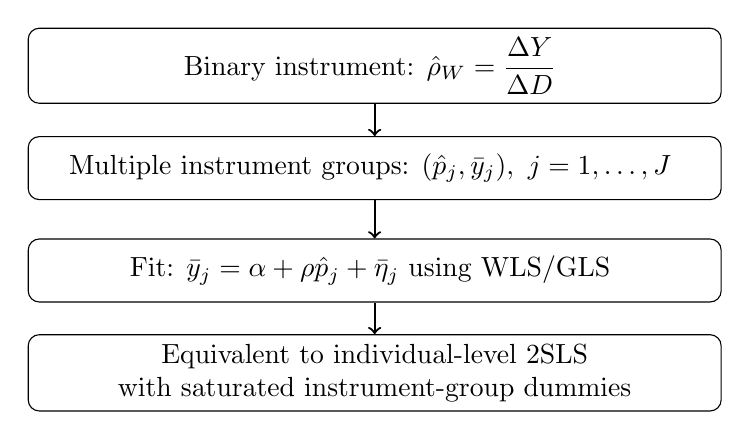
\begin{tikzpicture}[
    node distance=1.3cm,
    box/.style={
        rectangle,
        draw,
        rounded corners,
        minimum width=8.8cm,
        minimum height=0.8cm,
        align=center
    }
]

\node[box] (wald) {
Binary instrument:
\(\displaystyle
\hat\rho_W=\frac{\Delta Y}{\Delta D}
\)
};

\node[box, below of=wald] (groups) {
Multiple instrument groups:
\(\displaystyle
(\hat p_j,\bar y_j),\ j=1,\ldots,J
\)
};

\node[box, below of=groups] (gls) {
Fit:
\(\displaystyle
\bar y_j=\alpha+\rho\hat p_j+\bar\eta_j
\)
using WLS/GLS
};

\node[box, below of=gls] (twosls) {
Equivalent to individual-level 2SLS\\
with saturated instrument-group dummies
};

\draw[->, thick] (wald) -- (groups);
\draw[->, thick] (groups) -- (gls);
\draw[->, thick] (gls) -- (twosls);

\end{tikzpicture}
\end{center}

\end{frame}

% ================================================================
\begin{frame}{Main Takeaways}

\begin{enumerate}
    \item The Wald estimator is the basic building block of IV:
    \[
    \boxed{\text{Wald}=\frac{\Delta Y}{\Delta D}.}
    \]

    \item A multi-valued instrument generates many group-level Wald comparisons.

    \item Grouped data summarize each instrument cell by
    \[
    \left(
    \E[D\mid Z=z],
    \E[Y\mid Z=z]
    \right).
    \]

    \item Under constant treatment effects, these group means lie on a line whose slope is the causal effect.

    \item Grouped-data WLS is equivalent to 2SLS with saturated dummy instruments.

    \item Therefore,
    \[
    \boxed{
    \text{2SLS is an efficient way of combining instrument-induced causal comparisons.}
    }
    \]
\end{enumerate}

\end{frame}

% ================================================================
\begin{frame}{One-Sentence Summary}

\begin{center}

\vspace{0.8cm}

{\Large
\[
\boxed{
\text{2SLS regresses reduced-form variation}
\atop
\text{on first-stage variation.}
}
\]
}

\vspace{0.7cm}

Equivalently,

\[
\boxed{
\text{2SLS asks how much outcome variation is generated per unit of}
}
\]

\[
\boxed{
\text{instrument-induced treatment variation.}
}
\]

\end{center}

\end{frame}

% ================================================================
\begin{frame}{Reference}

\small

Angrist, J. D. (1990).\\
\textit{Lifetime Earnings and the Vietnam Era Draft Lottery: Evidence from Social Security Administrative Records}.\\
American Economic Review, 80(3), 313--336.

\vspace{0.5cm}

Angrist, J. D. and Pischke, J.-S.\\
\textit{Mostly Harmless Econometrics: An Empiricist's Companion}.\\
Chapter 4: Instrumental Variables in Action.

\vspace{0.5cm}

Section: \textit{Grouped Data and 2SLS}.

\end{frame}

% ================================================================
\end{document}
